\documentclass[]{article}
\usepackage{lmodern}
\usepackage{amssymb,amsmath}
\usepackage{ifxetex,ifluatex}
\usepackage{fixltx2e} % provides \textsubscript
\ifnum 0\ifxetex 1\fi\ifluatex 1\fi=0 % if pdftex
  \usepackage[T1]{fontenc}
  \usepackage[utf8]{inputenc}
\else % if luatex or xelatex
  \ifxetex
    \usepackage{mathspec}
  \else
    \usepackage{fontspec}
  \fi
  \defaultfontfeatures{Ligatures=TeX,Scale=MatchLowercase}
\fi
% use upquote if available, for straight quotes in verbatim environments
\IfFileExists{upquote.sty}{\usepackage{upquote}}{}
% use microtype if available
\IfFileExists{microtype.sty}{%
\usepackage{microtype}
\UseMicrotypeSet[protrusion]{basicmath} % disable protrusion for tt fonts
}{}
\usepackage[margin=1in]{geometry}
\usepackage{hyperref}
\hypersetup{unicode=true,
            pdfborder={0 0 0},
            breaklinks=true}
\urlstyle{same}  % don't use monospace font for urls
\usepackage{color}
\usepackage{fancyvrb}
\newcommand{\VerbBar}{|}
\newcommand{\VERB}{\Verb[commandchars=\\\{\}]}
\DefineVerbatimEnvironment{Highlighting}{Verbatim}{commandchars=\\\{\}}
% Add ',fontsize=\small' for more characters per line
\usepackage{framed}
\definecolor{shadecolor}{RGB}{248,248,248}
\newenvironment{Shaded}{\begin{snugshade}}{\end{snugshade}}
\newcommand{\KeywordTok}[1]{\textcolor[rgb]{0.13,0.29,0.53}{\textbf{#1}}}
\newcommand{\DataTypeTok}[1]{\textcolor[rgb]{0.13,0.29,0.53}{#1}}
\newcommand{\DecValTok}[1]{\textcolor[rgb]{0.00,0.00,0.81}{#1}}
\newcommand{\BaseNTok}[1]{\textcolor[rgb]{0.00,0.00,0.81}{#1}}
\newcommand{\FloatTok}[1]{\textcolor[rgb]{0.00,0.00,0.81}{#1}}
\newcommand{\ConstantTok}[1]{\textcolor[rgb]{0.00,0.00,0.00}{#1}}
\newcommand{\CharTok}[1]{\textcolor[rgb]{0.31,0.60,0.02}{#1}}
\newcommand{\SpecialCharTok}[1]{\textcolor[rgb]{0.00,0.00,0.00}{#1}}
\newcommand{\StringTok}[1]{\textcolor[rgb]{0.31,0.60,0.02}{#1}}
\newcommand{\VerbatimStringTok}[1]{\textcolor[rgb]{0.31,0.60,0.02}{#1}}
\newcommand{\SpecialStringTok}[1]{\textcolor[rgb]{0.31,0.60,0.02}{#1}}
\newcommand{\ImportTok}[1]{#1}
\newcommand{\CommentTok}[1]{\textcolor[rgb]{0.56,0.35,0.01}{\textit{#1}}}
\newcommand{\DocumentationTok}[1]{\textcolor[rgb]{0.56,0.35,0.01}{\textbf{\textit{#1}}}}
\newcommand{\AnnotationTok}[1]{\textcolor[rgb]{0.56,0.35,0.01}{\textbf{\textit{#1}}}}
\newcommand{\CommentVarTok}[1]{\textcolor[rgb]{0.56,0.35,0.01}{\textbf{\textit{#1}}}}
\newcommand{\OtherTok}[1]{\textcolor[rgb]{0.56,0.35,0.01}{#1}}
\newcommand{\FunctionTok}[1]{\textcolor[rgb]{0.00,0.00,0.00}{#1}}
\newcommand{\VariableTok}[1]{\textcolor[rgb]{0.00,0.00,0.00}{#1}}
\newcommand{\ControlFlowTok}[1]{\textcolor[rgb]{0.13,0.29,0.53}{\textbf{#1}}}
\newcommand{\OperatorTok}[1]{\textcolor[rgb]{0.81,0.36,0.00}{\textbf{#1}}}
\newcommand{\BuiltInTok}[1]{#1}
\newcommand{\ExtensionTok}[1]{#1}
\newcommand{\PreprocessorTok}[1]{\textcolor[rgb]{0.56,0.35,0.01}{\textit{#1}}}
\newcommand{\AttributeTok}[1]{\textcolor[rgb]{0.77,0.63,0.00}{#1}}
\newcommand{\RegionMarkerTok}[1]{#1}
\newcommand{\InformationTok}[1]{\textcolor[rgb]{0.56,0.35,0.01}{\textbf{\textit{#1}}}}
\newcommand{\WarningTok}[1]{\textcolor[rgb]{0.56,0.35,0.01}{\textbf{\textit{#1}}}}
\newcommand{\AlertTok}[1]{\textcolor[rgb]{0.94,0.16,0.16}{#1}}
\newcommand{\ErrorTok}[1]{\textcolor[rgb]{0.64,0.00,0.00}{\textbf{#1}}}
\newcommand{\NormalTok}[1]{#1}
\usepackage{graphicx,grffile}
\makeatletter
\def\maxwidth{\ifdim\Gin@nat@width>\linewidth\linewidth\else\Gin@nat@width\fi}
\def\maxheight{\ifdim\Gin@nat@height>\textheight\textheight\else\Gin@nat@height\fi}
\makeatother
% Scale images if necessary, so that they will not overflow the page
% margins by default, and it is still possible to overwrite the defaults
% using explicit options in \includegraphics[width, height, ...]{}
\setkeys{Gin}{width=\maxwidth,height=\maxheight,keepaspectratio}
\IfFileExists{parskip.sty}{%
\usepackage{parskip}
}{% else
\setlength{\parindent}{0pt}
\setlength{\parskip}{6pt plus 2pt minus 1pt}
}
\setlength{\emergencystretch}{3em}  % prevent overfull lines
\providecommand{\tightlist}{%
  \setlength{\itemsep}{0pt}\setlength{\parskip}{0pt}}
\setcounter{secnumdepth}{0}
% Redefines (sub)paragraphs to behave more like sections
\ifx\paragraph\undefined\else
\let\oldparagraph\paragraph
\renewcommand{\paragraph}[1]{\oldparagraph{#1}\mbox{}}
\fi
\ifx\subparagraph\undefined\else
\let\oldsubparagraph\subparagraph
\renewcommand{\subparagraph}[1]{\oldsubparagraph{#1}\mbox{}}
\fi

%%% Use protect on footnotes to avoid problems with footnotes in titles
\let\rmarkdownfootnote\footnote%
\def\footnote{\protect\rmarkdownfootnote}

%%% Change title format to be more compact
\usepackage{titling}

% Create subtitle command for use in maketitle
\newcommand{\subtitle}[1]{
  \posttitle{
    \begin{center}\large#1\end{center}
    }
}

\setlength{\droptitle}{-2em}

  \title{}
    \pretitle{\vspace{\droptitle}}
  \posttitle{}
    \author{}
    \preauthor{}\postauthor{}
    \date{}
    \predate{}\postdate{}
  

\begin{document}

\begin{Shaded}
\begin{Highlighting}[]
\NormalTok{knitr}\OperatorTok{::}\NormalTok{opts_chunk}\OperatorTok{$}\KeywordTok{set}\NormalTok{(}\DataTypeTok{echo =} \OtherTok{TRUE}\NormalTok{)}
\NormalTok{nsims <-}\StringTok{ }\DecValTok{100000} \CommentTok{#set number of simulations}
\KeywordTok{require}\NormalTok{(mvtnorm, }\DataTypeTok{quietly =} \OtherTok{TRUE}\NormalTok{)}
\KeywordTok{require}\NormalTok{(MASS, }\DataTypeTok{quietly =} \OtherTok{TRUE}\NormalTok{)}
\KeywordTok{require}\NormalTok{(afex, }\DataTypeTok{quietly =} \OtherTok{TRUE}\NormalTok{)}
\KeywordTok{require}\NormalTok{(emmeans, }\DataTypeTok{quietly =} \OtherTok{TRUE}\NormalTok{)}
\KeywordTok{require}\NormalTok{(ggplot2, }\DataTypeTok{quietly =} \OtherTok{TRUE}\NormalTok{)}
\KeywordTok{require}\NormalTok{(gridExtra, }\DataTypeTok{quietly =} \OtherTok{TRUE}\NormalTok{)}
\KeywordTok{require}\NormalTok{(reshape2, }\DataTypeTok{quietly =} \OtherTok{TRUE}\NormalTok{)}
\KeywordTok{require}\NormalTok{(pwr, }\DataTypeTok{quietly =} \OtherTok{TRUE}\NormalTok{)}

\CommentTok{# Install functions from GitHub by running the code below:}
\KeywordTok{source}\NormalTok{(}\StringTok{"https://raw.githubusercontent.com/Lakens/ANOVA_power_simulation/master/ANOVA_design.R"}\NormalTok{)}
\KeywordTok{source}\NormalTok{(}\StringTok{"https://raw.githubusercontent.com/Lakens/ANOVA_power_simulation/master/ANOVA_power.R"}\NormalTok{)}
\end{Highlighting}
\end{Shaded}

\subsection{Power in Interactions}\label{power-in-interactions}

In the 17th Data Colada blog post titles
\href{http://datacolada.org/17}{No-way Interactions} Uri Simonsohn
discusses how a moderated interaction (the effect is there in one
condition, but disappears in another condition) requires at least twice
as many subjects per cell as a study that simply aims to show the simple
effect. For example, see the plot below. Assume the score on the
vertical axis is desire for fruit, as a function of the fruit that is
available (an apple or a banana) and how hungry people are (not, or
very). We see there is a difference between the participants desire for
a banana compared to an apple, but only for participants who are very
hungry. The point that is made is that you need twice as many
participants in each cell to have power for the interaction, as you need
for the simple effect.

\begin{Shaded}
\begin{Highlighting}[]
\NormalTok{string <-}\StringTok{ "2b*2b"}
\NormalTok{n <-}\StringTok{ }\DecValTok{20}
\NormalTok{mu <-}\StringTok{ }\KeywordTok{c}\NormalTok{(}\DecValTok{20}\NormalTok{, }\DecValTok{20}\NormalTok{, }\DecValTok{20}\NormalTok{, }\DecValTok{25}\NormalTok{) }\CommentTok{#All means are equal - so there is no real difference.}
\CommentTok{# Enter means in the order that matches the labels below.}
\NormalTok{sd <-}\StringTok{ }\FloatTok{0.5}
\NormalTok{labelnames <-}\StringTok{ }\KeywordTok{c}\NormalTok{(}\StringTok{"fruit"}\NormalTok{, }\StringTok{"apple"}\NormalTok{, }\StringTok{"banana"}\NormalTok{, }\StringTok{"hunger"}\NormalTok{, }\StringTok{"no hunger"}\NormalTok{, }\StringTok{"very hungry"}\NormalTok{) }\CommentTok{#}
\CommentTok{# the label names should be in the order of the means specified above.}

\NormalTok{design_result <-}\StringTok{ }\KeywordTok{ANOVA_design}\NormalTok{(}\DataTypeTok{string =}\NormalTok{ string,}
                   \DataTypeTok{n =}\NormalTok{ n, }
                   \DataTypeTok{mu =}\NormalTok{ mu, }
                   \DataTypeTok{sd =}\NormalTok{ sd, }
                   \DataTypeTok{labelnames =}\NormalTok{ labelnames)}
\end{Highlighting}
\end{Shaded}

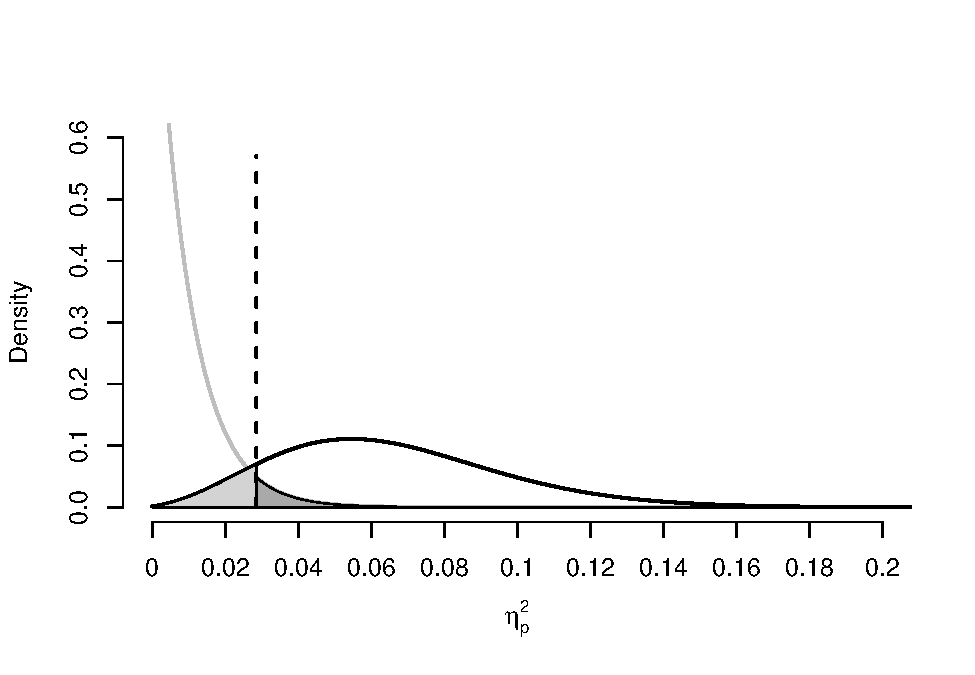
\includegraphics{4.2_power_for_interactions_files/figure-latex/unnamed-chunk-1-1.pdf}

We can reproduce the simulations in the Data Colada blog post, using the
original code.

\begin{Shaded}
\begin{Highlighting}[]
\CommentTok{#R-Code}
\CommentTok{#}
\CommentTok{#Written by Uri Simonsohn, March 2014}
\CommentTok{#}
\CommentTok{#}
\CommentTok{#In DataColada[17] I propose that 2x2 interaction studies need 2x the sample size}
\CommentTok{#http://datacolada.org/2014/03/10/17-no-way-interactions}
\CommentTok{#In a companion ,pdf I show the simple math behind it}
\CommentTok{#}
\CommentTok{#}
\CommentTok{#Simulations are often more persuasive than math, so here it goes.}
\CommentTok{#I run simulations that compute power for 2 and 4 cell design, the latter testing the interaction}
\NormalTok{###################################################################################################}

\CommentTok{#Create function that computes power of Studies 1 and 2, where Study 1  has 2 cells and tests a simple effect}
\CommentTok{#and Study 2 has 4 cells and tests the interaction}

\NormalTok{  colada17=}\ControlFlowTok{function}\NormalTok{(d1,d2,n1,n2,simtot)}
\NormalTok{  \{}
  \CommentTok{#n1: sample size, per cell, study 1}
  \CommentTok{#n2: sample size, per cell, study 2}
  \CommentTok{#d1: simple effect M1-M2}
  \CommentTok{#d2: moderated effect M3-M4, full elimination of effect implies d2=0}
  \CommentTok{#simtot: how many simulations to run}


  \CommentTok{#Here we will store results}
\NormalTok{      p1=}\KeywordTok{c}\NormalTok{()    }\CommentTok{#p-values for Study 1}
\NormalTok{      p2=}\KeywordTok{c}\NormalTok{()    }\CommentTok{#p-values for Study 2}


  \ControlFlowTok{for}\NormalTok{(i }\ControlFlowTok{in} \DecValTok{1}\OperatorTok{:}\NormalTok{simtot) \{}
    \CommentTok{#draw data 4 samples}
\NormalTok{    y1=}\KeywordTok{rnorm}\NormalTok{(}\DataTypeTok{n=}\KeywordTok{max}\NormalTok{(n1,n2),}\DataTypeTok{mean=}\NormalTok{d1)}
\NormalTok{    y2=}\KeywordTok{rnorm}\NormalTok{(}\DataTypeTok{n=}\KeywordTok{max}\NormalTok{(n1,n2))}
\NormalTok{    y3=}\KeywordTok{rnorm}\NormalTok{(}\DataTypeTok{n=}\KeywordTok{max}\NormalTok{(n1,n2),}\DataTypeTok{mean=}\NormalTok{d2)}
\NormalTok{    y4=}\KeywordTok{rnorm}\NormalTok{(}\DataTypeTok{n=}\KeywordTok{max}\NormalTok{(n1,n2))}
    
    \CommentTok{#GET DATA READY FOR ANOVA  }
\NormalTok{      y=}\KeywordTok{c}\NormalTok{(y1,y2,y3,y4)          }\CommentTok{#the d.v.}
\NormalTok{      nrep=}\KeywordTok{rep}\NormalTok{(n2,}\DecValTok{4}\NormalTok{)          }
\NormalTok{      A=}\KeywordTok{rep}\NormalTok{(}\KeywordTok{c}\NormalTok{(}\DecValTok{1}\NormalTok{,}\DecValTok{1}\NormalTok{,}\DecValTok{0}\NormalTok{,}\DecValTok{0}\NormalTok{),}\DataTypeTok{times=}\NormalTok{nrep) }
\NormalTok{      B=}\KeywordTok{rep}\NormalTok{(}\KeywordTok{c}\NormalTok{(}\DecValTok{1}\NormalTok{,}\DecValTok{0}\NormalTok{,}\DecValTok{1}\NormalTok{,}\DecValTok{0}\NormalTok{),}\DataTypeTok{times=}\NormalTok{nrep)}
    
    \CommentTok{#STUDY 1}
\NormalTok{      p1.k=}\KeywordTok{t.test}\NormalTok{(y1[}\DecValTok{1}\OperatorTok{:}\NormalTok{n1],y2[}\DecValTok{1}\OperatorTok{:}\NormalTok{n1],}\DataTypeTok{var.equal=}\OtherTok{TRUE}\NormalTok{)}\OperatorTok{$}\NormalTok{p.value  }\CommentTok{#Do a t-test on the first n1 observations}
    
    \CommentTok{#STUDY 2}
\NormalTok{      p2.k=}\KeywordTok{anova}\NormalTok{(}\KeywordTok{lm}\NormalTok{(y }\OperatorTok{~}\StringTok{ }\NormalTok{A }\OperatorTok{*}\StringTok{ }\NormalTok{B))[}\StringTok{"A:B"}\NormalTok{, }\StringTok{"Pr(>F)"}\NormalTok{]             }\CommentTok{#Do anova, keep p-value of the interaction}
        
      \CommentTok{#Store the results}
\NormalTok{      p1=}\KeywordTok{c}\NormalTok{(p1,p1.k)}
\NormalTok{      p2=}\KeywordTok{c}\NormalTok{(p2,p2.k)}
    
\NormalTok{      \}}
  
  \CommentTok{#What share off comparisons are significant}
\NormalTok{    power1=}\KeywordTok{sum}\NormalTok{(p1}\OperatorTok{<=}\NormalTok{.}\DecValTok{05}\NormalTok{)}\OperatorTok{/}\NormalTok{simtot  }\CommentTok{#Simple test using estimate of variance from 2 cells only}
\NormalTok{    power2=}\KeywordTok{sum}\NormalTok{(p2}\OperatorTok{<=}\NormalTok{.}\DecValTok{05}\NormalTok{)}\OperatorTok{/}\NormalTok{simtot  }\CommentTok{#Interaction}
  
    \KeywordTok{cat}\NormalTok{(}\StringTok{"}\CharTok{\textbackslash{}n}\StringTok{Study 1 is powered to:"}\NormalTok{,}\KeywordTok{round}\NormalTok{(power1,}\DecValTok{2}\NormalTok{))}
    \KeywordTok{cat}\NormalTok{(}\StringTok{"}\CharTok{\textbackslash{}n}\StringTok{Study 2 is powered to:"}\NormalTok{,}\KeywordTok{round}\NormalTok{(power2,}\DecValTok{2}\NormalTok{))}
  
\NormalTok{    \}}
    
    

\CommentTok{#Same power for 2n regardless of n and d}
  \KeywordTok{colada17}\NormalTok{(}\DataTypeTok{simtot=}\DecValTok{2000}\NormalTok{, }\DataTypeTok{n1=}\DecValTok{20}\NormalTok{,}\DataTypeTok{n2=}\DecValTok{40}\NormalTok{,}\DataTypeTok{d1=}\DecValTok{1}\NormalTok{,}\DataTypeTok{d2=}\DecValTok{0}\NormalTok{)  }
\end{Highlighting}
\end{Shaded}

\begin{verbatim}
## 
## Study 1 is powered to: 0.86
## Study 2 is powered to: 0.87
\end{verbatim}

\begin{Shaded}
\begin{Highlighting}[]
  \KeywordTok{colada17}\NormalTok{(}\DataTypeTok{simtot=}\DecValTok{2000}\NormalTok{, }\DataTypeTok{n1=}\DecValTok{50}\NormalTok{,}\DataTypeTok{n2=}\DecValTok{100}\NormalTok{,}\DataTypeTok{d1=}\NormalTok{.}\DecValTok{3}\NormalTok{,}\DataTypeTok{d2=}\DecValTok{0}\NormalTok{)}
\end{Highlighting}
\end{Shaded}

\begin{verbatim}
## 
## Study 1 is powered to: 0.31
## Study 2 is powered to: 0.32
\end{verbatim}

\begin{Shaded}
\begin{Highlighting}[]
  \KeywordTok{colada17}\NormalTok{(}\DataTypeTok{simtot=}\DecValTok{2000}\NormalTok{, }\DataTypeTok{n1=}\DecValTok{150}\NormalTok{,}\DataTypeTok{n2=}\DecValTok{300}\NormalTok{,}\DataTypeTok{d1=}\NormalTok{.}\DecValTok{25}\NormalTok{,}\DataTypeTok{d2=}\DecValTok{0}\NormalTok{)}
\end{Highlighting}
\end{Shaded}

\begin{verbatim}
## 
## Study 1 is powered to: 0.59
## Study 2 is powered to: 0.57
\end{verbatim}

\begin{Shaded}
\begin{Highlighting}[]
\CommentTok{#Need 4n if effect is 70% attenuated}
  \KeywordTok{colada17}\NormalTok{(}\DataTypeTok{simtot=}\DecValTok{2000}\NormalTok{, }\DataTypeTok{n1=}\DecValTok{25}\NormalTok{,}\DataTypeTok{n2=}\DecValTok{100}\NormalTok{,}\DataTypeTok{d1=}\NormalTok{.}\DecValTok{5}\NormalTok{, }\DataTypeTok{d2=}\NormalTok{.}\DecValTok{3}\OperatorTok{*}\NormalTok{.}\DecValTok{5}\NormalTok{)}
\end{Highlighting}
\end{Shaded}

\begin{verbatim}
## 
## Study 1 is powered to: 0.41
## Study 2 is powered to: 0.42
\end{verbatim}

\begin{Shaded}
\begin{Highlighting}[]
  \KeywordTok{colada17}\NormalTok{(}\DataTypeTok{simtot=}\DecValTok{2000}\NormalTok{, }\DataTypeTok{n1=}\DecValTok{50}\NormalTok{,}\DataTypeTok{n2=}\DecValTok{200}\NormalTok{,}\DataTypeTok{d1=}\NormalTok{.}\DecValTok{5}\NormalTok{, }\DataTypeTok{d2=}\NormalTok{.}\DecValTok{3}\OperatorTok{*}\NormalTok{.}\DecValTok{5}\NormalTok{)}
\end{Highlighting}
\end{Shaded}

\begin{verbatim}
## 
## Study 1 is powered to: 0.7
## Study 2 is powered to: 0.7
\end{verbatim}

\begin{Shaded}
\begin{Highlighting}[]
  \KeywordTok{colada17}\NormalTok{(}\DataTypeTok{simtot=}\DecValTok{2000}\NormalTok{, }\DataTypeTok{n1=}\DecValTok{22}\NormalTok{,}\DataTypeTok{n2=}\DecValTok{88}\NormalTok{,}\DataTypeTok{d1=}\NormalTok{.}\DecValTok{41}\NormalTok{, }\DataTypeTok{d2=}\NormalTok{.}\DecValTok{3}\OperatorTok{*}\NormalTok{.}\DecValTok{41}\NormalTok{)}
\end{Highlighting}
\end{Shaded}

\begin{verbatim}
## 
## Study 1 is powered to: 0.25
## Study 2 is powered to: 0.28
\end{verbatim}

\begin{Shaded}
\begin{Highlighting}[]
\CommentTok{#underpowered if run with the same n}
\KeywordTok{colada17}\NormalTok{(}\DataTypeTok{simtot=}\NormalTok{nsims, }\DataTypeTok{n1=}\DecValTok{20}\NormalTok{,}\DataTypeTok{n2=}\DecValTok{20}\NormalTok{,}\DataTypeTok{d1=}\DecValTok{1}\NormalTok{,}\DataTypeTok{d2=}\DecValTok{0}\NormalTok{)  }
\end{Highlighting}
\end{Shaded}

\begin{verbatim}
## 
## Study 1 is powered to: 0.87
## Study 2 is powered to: 0.6
\end{verbatim}

And we can reproduce the results using the ANOVA\_power function.

\begin{Shaded}
\begin{Highlighting}[]
\NormalTok{alpha_level <-}\StringTok{ }\FloatTok{0.05} \CommentTok{#We set the alpha level at 0.05. }

\NormalTok{power_result <-}\StringTok{ }\KeywordTok{ANOVA_power}\NormalTok{(design_result, }\DataTypeTok{alpha_level =}\NormalTok{ alpha_level, }\DataTypeTok{nsims =}\NormalTok{ nsims)}
\end{Highlighting}
\end{Shaded}

\begin{verbatim}
## Power and Effect sizes for ANOVA tests
##                    power effect size
## anova_fruit          100      0.8691
## anova_hunger         100      0.8689
## anova_fruit:hunger   100      0.8690
## 
## Power and Effect sizes for contrasts
##                                                                    power
## p_fruit_apple_hunger_no hunger_fruit_apple_hunger_very hungry      5.031
## p_fruit_apple_hunger_no hunger_fruit_banana_hunger_no hunger       4.902
## p_fruit_apple_hunger_no hunger_fruit_banana_hunger_very hungry   100.000
## p_fruit_apple_hunger_very hungry_fruit_banana_hunger_no hunger     5.025
## p_fruit_apple_hunger_very hungry_fruit_banana_hunger_very hungry 100.000
## p_fruit_banana_hunger_no hunger_fruit_banana_hunger_very hungry  100.000
##                                                                  effect size
## p_fruit_apple_hunger_no hunger_fruit_apple_hunger_very hungry        -0.0004
## p_fruit_apple_hunger_no hunger_fruit_banana_hunger_no hunger          0.0012
## p_fruit_apple_hunger_no hunger_fruit_banana_hunger_very hungry       10.2028
## p_fruit_apple_hunger_very hungry_fruit_banana_hunger_no hunger        0.0017
## p_fruit_apple_hunger_very hungry_fruit_banana_hunger_very hungry     10.2037
## p_fruit_banana_hunger_no hunger_fruit_banana_hunger_very hungry      10.2001
\end{verbatim}

We see we get the same power for the anova\_fruit:hunger interaction and
for the simple effect p\_fruit\_apple\_hunger\_very
hungry\_fruit\_banana\_hunger\_very hungry as the simulations by Uri
Simonsohn in his blog post.

\begin{Shaded}
\begin{Highlighting}[]
\CommentTok{#Same power for 2n regardless of n and d}
  \KeywordTok{colada17}\NormalTok{(}\DataTypeTok{simtot=}\DecValTok{10000}\NormalTok{, }\DataTypeTok{n1=}\DecValTok{20}\NormalTok{,}\DataTypeTok{n2=}\DecValTok{40}\NormalTok{,}\DataTypeTok{d1=}\DecValTok{1}\NormalTok{,}\DataTypeTok{d2=}\DecValTok{0}\NormalTok{)  }
\end{Highlighting}
\end{Shaded}

\begin{verbatim}
## 
## Study 1 is powered to: 0.87
## Study 2 is powered to: 0.88
\end{verbatim}

\begin{Shaded}
\begin{Highlighting}[]
  \KeywordTok{colada17}\NormalTok{(}\DataTypeTok{simtot=}\DecValTok{10000}\NormalTok{, }\DataTypeTok{n1=}\DecValTok{50}\NormalTok{,}\DataTypeTok{n2=}\DecValTok{100}\NormalTok{,}\DataTypeTok{d1=}\NormalTok{.}\DecValTok{3}\NormalTok{,}\DataTypeTok{d2=}\DecValTok{0}\NormalTok{)}
\end{Highlighting}
\end{Shaded}

\begin{verbatim}
## 
## Study 1 is powered to: 0.31
## Study 2 is powered to: 0.32
\end{verbatim}

\begin{Shaded}
\begin{Highlighting}[]
  \KeywordTok{colada17}\NormalTok{(}\DataTypeTok{simtot=}\DecValTok{10000}\NormalTok{, }\DataTypeTok{n1=}\DecValTok{150}\NormalTok{,}\DataTypeTok{n2=}\DecValTok{300}\NormalTok{,}\DataTypeTok{d1=}\NormalTok{.}\DecValTok{25}\NormalTok{,}\DataTypeTok{d2=}\DecValTok{0}\NormalTok{)}
\end{Highlighting}
\end{Shaded}

\begin{verbatim}
## 
## Study 1 is powered to: 0.58
## Study 2 is powered to: 0.59
\end{verbatim}

We can also reproduce the last example by adjusting the means and
standard deviation. With 150 people, and a Cohen's d of 0.25 (the
difference is 5, the sd 20, so 5/20 = 0.25) we should reproduce the
power for the simple effect.

\begin{Shaded}
\begin{Highlighting}[]
\NormalTok{string <-}\StringTok{ "2b*2b"}
\NormalTok{n <-}\StringTok{ }\DecValTok{150}
\NormalTok{mu <-}\StringTok{ }\KeywordTok{c}\NormalTok{(}\DecValTok{20}\NormalTok{, }\DecValTok{20}\NormalTok{, }\DecValTok{20}\NormalTok{, }\DecValTok{25}\NormalTok{) }\CommentTok{#All means are equal - so there is no real difference.}
\CommentTok{# Enter means in the order that matches the labels below.}
\NormalTok{sd <-}\StringTok{ }\DecValTok{20}
\NormalTok{labelnames <-}\StringTok{ }\KeywordTok{c}\NormalTok{(}\StringTok{"fruit"}\NormalTok{, }\StringTok{"apple"}\NormalTok{, }\StringTok{"banana"}\NormalTok{, }\StringTok{"hunger"}\NormalTok{, }\StringTok{"no hunger"}\NormalTok{, }\StringTok{"very hungry"}\NormalTok{) }\CommentTok{#}
\CommentTok{# the label names should be in the order of the means specified above.}

\NormalTok{design_result <-}\StringTok{ }\KeywordTok{ANOVA_design}\NormalTok{(}\DataTypeTok{string =}\NormalTok{ string,}
                   \DataTypeTok{n =}\NormalTok{ n, }
                   \DataTypeTok{mu =}\NormalTok{ mu, }
                   \DataTypeTok{sd =}\NormalTok{ sd, }
                   \DataTypeTok{labelnames =}\NormalTok{ labelnames)}
\end{Highlighting}
\end{Shaded}

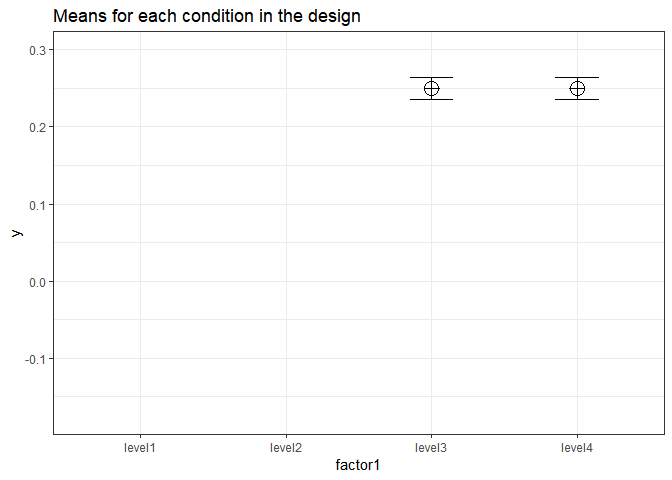
\includegraphics{4.2_power_for_interactions_files/figure-latex/unnamed-chunk-6-1.pdf}

\begin{Shaded}
\begin{Highlighting}[]
\NormalTok{alpha_level <-}\StringTok{ }\FloatTok{0.05} \CommentTok{#We set the alpha level at 0.05. }

\NormalTok{power_result <-}\StringTok{ }\KeywordTok{ANOVA_power}\NormalTok{(design_result, }\DataTypeTok{alpha_level =}\NormalTok{ alpha_level, }\DataTypeTok{nsims =}\NormalTok{ nsims)}
\end{Highlighting}
\end{Shaded}

\begin{verbatim}
## Power and Effect sizes for ANOVA tests
##                     power effect size
## anova_fruit        33.214      0.0039
## anova_hunger       33.408      0.0039
## anova_fruit:hunger 33.130      0.0039
## 
## Power and Effect sizes for contrasts
##                                                                   power
## p_fruit_apple_hunger_no hunger_fruit_apple_hunger_very hungry     4.955
## p_fruit_apple_hunger_no hunger_fruit_banana_hunger_no hunger      4.997
## p_fruit_apple_hunger_no hunger_fruit_banana_hunger_very hungry   57.784
## p_fruit_apple_hunger_very hungry_fruit_banana_hunger_no hunger    4.946
## p_fruit_apple_hunger_very hungry_fruit_banana_hunger_very hungry 58.085
## p_fruit_banana_hunger_no hunger_fruit_banana_hunger_very hungry  57.838
##                                                                  effect size
## p_fruit_apple_hunger_no hunger_fruit_apple_hunger_very hungry        -0.0001
## p_fruit_apple_hunger_no hunger_fruit_banana_hunger_no hunger          0.0000
## p_fruit_apple_hunger_no hunger_fruit_banana_hunger_very hungry        0.2505
## p_fruit_apple_hunger_very hungry_fruit_banana_hunger_no hunger        0.0001
## p_fruit_apple_hunger_very hungry_fruit_banana_hunger_very hungry      0.2505
## p_fruit_banana_hunger_no hunger_fruit_banana_hunger_very hungry       0.2505
\end{verbatim}

And changing the sample size to 300 should reproduce the power for the
interaction in the ANOVA.

\begin{Shaded}
\begin{Highlighting}[]
\NormalTok{string <-}\StringTok{ "2b*2b"}
\NormalTok{n <-}\StringTok{ }\DecValTok{300}
\NormalTok{mu <-}\StringTok{ }\KeywordTok{c}\NormalTok{(}\DecValTok{20}\NormalTok{, }\DecValTok{20}\NormalTok{, }\DecValTok{20}\NormalTok{, }\DecValTok{25}\NormalTok{) }\CommentTok{#All means are equal - so there is no real difference.}
\CommentTok{# Enter means in the order that matches the labels below.}
\NormalTok{sd <-}\StringTok{ }\DecValTok{20}
\NormalTok{labelnames <-}\StringTok{ }\KeywordTok{c}\NormalTok{(}\StringTok{"fruit"}\NormalTok{, }\StringTok{"apple"}\NormalTok{, }\StringTok{"banana"}\NormalTok{, }\StringTok{"hunger"}\NormalTok{, }\StringTok{"no hunger"}\NormalTok{, }\StringTok{"very hungry"}\NormalTok{) }\CommentTok{#}
\CommentTok{# the label names should be in the order of the means specified above.}

\NormalTok{design_result <-}\StringTok{ }\KeywordTok{ANOVA_design}\NormalTok{(}\DataTypeTok{string =}\NormalTok{ string,}
                   \DataTypeTok{n =}\NormalTok{ n, }
                   \DataTypeTok{mu =}\NormalTok{ mu, }
                   \DataTypeTok{sd =}\NormalTok{ sd, }
                   \DataTypeTok{labelnames =}\NormalTok{ labelnames)}
\end{Highlighting}
\end{Shaded}

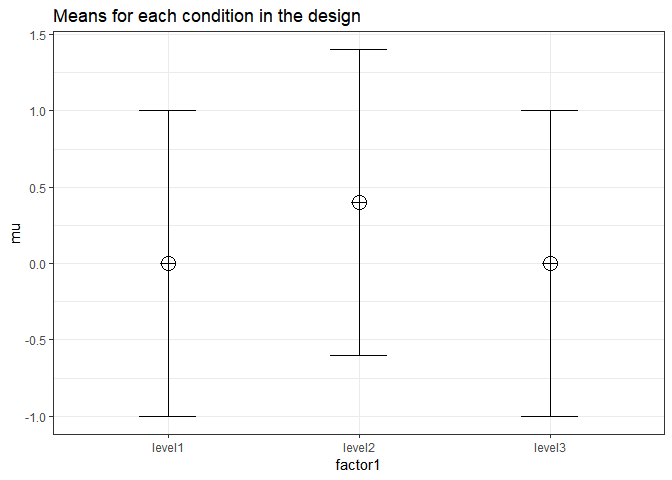
\includegraphics{4.2_power_for_interactions_files/figure-latex/unnamed-chunk-7-1.pdf}

\begin{Shaded}
\begin{Highlighting}[]
\NormalTok{alpha_level <-}\StringTok{ }\FloatTok{0.05} \CommentTok{#We set the alpha level at 0.05. }

\NormalTok{power_result <-}\StringTok{ }\KeywordTok{ANOVA_power}\NormalTok{(design_result, }\DataTypeTok{alpha_level =}\NormalTok{ alpha_level, }\DataTypeTok{nsims =}\NormalTok{ nsims)}
\end{Highlighting}
\end{Shaded}

\begin{verbatim}
## Power and Effect sizes for ANOVA tests
##                     power effect size
## anova_fruit        58.063      0.0039
## anova_hunger       57.820      0.0039
## anova_fruit:hunger 58.007      0.0039
## 
## Power and Effect sizes for contrasts
##                                                                   power
## p_fruit_apple_hunger_no hunger_fruit_apple_hunger_very hungry     4.961
## p_fruit_apple_hunger_no hunger_fruit_banana_hunger_no hunger      5.102
## p_fruit_apple_hunger_no hunger_fruit_banana_hunger_very hungry   86.342
## p_fruit_apple_hunger_very hungry_fruit_banana_hunger_no hunger    4.969
## p_fruit_apple_hunger_very hungry_fruit_banana_hunger_very hungry 86.327
## p_fruit_banana_hunger_no hunger_fruit_banana_hunger_very hungry  86.322
##                                                                  effect size
## p_fruit_apple_hunger_no hunger_fruit_apple_hunger_very hungry        -0.0002
## p_fruit_apple_hunger_no hunger_fruit_banana_hunger_no hunger          0.0001
## p_fruit_apple_hunger_no hunger_fruit_banana_hunger_very hungry        0.2499
## p_fruit_apple_hunger_very hungry_fruit_banana_hunger_no hunger        0.0003
## p_fruit_apple_hunger_very hungry_fruit_banana_hunger_very hungry      0.2502
## p_fruit_banana_hunger_no hunger_fruit_banana_hunger_very hungry       0.2499
\end{verbatim}

Now if we look at the power analysis table for the last simulation, we
see that the power for the ANOVA is the same for the main effect of
fruit, the main effect of hunger, and the main effect of the
interaction. All the effect sizes are equal as well. We can understand
why if we look at the means in a 2x2 table:

\begin{Shaded}
\begin{Highlighting}[]
\NormalTok{mean_mat <-}\StringTok{ }\KeywordTok{t}\NormalTok{(}\KeywordTok{matrix}\NormalTok{(mu, }
                     \DataTypeTok{nrow =} \DecValTok{2}\NormalTok{,}
                     \DataTypeTok{ncol =} \DecValTok{2}\NormalTok{)) }\CommentTok{#Create a mean matrix}
\KeywordTok{rownames}\NormalTok{(mean_mat) <-}\StringTok{ }\KeywordTok{c}\NormalTok{(}\StringTok{"apple"}\NormalTok{, }\StringTok{"banana"}\NormalTok{)}
\KeywordTok{colnames}\NormalTok{(mean_mat) <-}\StringTok{ }\KeywordTok{c}\NormalTok{(}\StringTok{"no hunger"}\NormalTok{, }\StringTok{"very hungry"}\NormalTok{)}
\NormalTok{mean_mat}
\end{Highlighting}
\end{Shaded}

\begin{verbatim}
##        no hunger very hungry
## apple         20          20
## banana        20          25
\end{verbatim}

The first main effect tests the marginal means if we sum over rows, 22.5
vs 20.

\begin{Shaded}
\begin{Highlighting}[]
\KeywordTok{rowMeans}\NormalTok{(mean_mat)}
\end{Highlighting}
\end{Shaded}

\begin{verbatim}
##  apple banana 
##   20.0   22.5
\end{verbatim}

The second main effect tests the marginal means over the rows, which is
also 22.5 vs 20.

\begin{Shaded}
\begin{Highlighting}[]
\KeywordTok{colMeans}\NormalTok{(mean_mat)}
\end{Highlighting}
\end{Shaded}

\begin{verbatim}
##   no hunger very hungry 
##        20.0        22.5
\end{verbatim}

The interaction tests whether the average effect of hunger on liking
fruit differs in the presence of bananas. In the presence of bananas the
effect of hunger on the desireability of fruit is 5 scalepoints. The
average effect (that we get from the marginal means) of hunger on fruit
desireability is 2.5 (22.5-20). In other words, the interaction tests
whether the difference effect between hunger and no hunger is different
in the presence of an apple versus in the presence of a banana.

Mathematically the interaction effect is computed as the difference
between a cell mean and the grand mean, the marginal mean in row i and
the grand mean, and the marginal mean in column j and grand mean. For
example, for the very hungry-banana condition this is 25 (the value in
the cell) - (21.25 {[}the grand mean{]} + 1.25 {[}the marginal mean in
row 2, 22.5, minus the grand mean of 21.25{]} + 1.25 {[}the marginal
mean in column 2, 22.5, minus the grand mean of 21.25{]}). 25 - (21.25 +
(22.5-21.25) + (22.5-21.25)) = 1.25.

We can repeat this for every cell, and get for no hunger-apple: 20 -
(21.25 + (20-21.25) + (20-21.25)) = 1.25, for very hungry apple: 20 -
(21.25 + (22.5-21.25) + (20-21.25)) = 1.25, and no hunger-banana: 20 -
(21.25 + (20-21.25) + (22.5-21.25)) = 1.25. These values are used to
calculate the sum of squares.

\begin{Shaded}
\begin{Highlighting}[]
\NormalTok{a1 <-}\StringTok{ }\NormalTok{mean_mat[}\DecValTok{1}\NormalTok{,}\DecValTok{1}\NormalTok{] }\OperatorTok{-}\StringTok{ }\NormalTok{(}\KeywordTok{mean}\NormalTok{(mean_mat) }\OperatorTok{+}\StringTok{ }\NormalTok{(}\KeywordTok{mean}\NormalTok{(mean_mat[}\DecValTok{1}\NormalTok{,]) }\OperatorTok{-}\StringTok{ }\KeywordTok{mean}\NormalTok{(mean_mat)) }\OperatorTok{+}\StringTok{ }\NormalTok{(}\KeywordTok{mean}\NormalTok{(mean_mat[,}\DecValTok{1}\NormalTok{]) }\OperatorTok{-}\StringTok{ }\KeywordTok{mean}\NormalTok{(mean_mat)))}
\NormalTok{a2 <-}\StringTok{ }\NormalTok{mean_mat[}\DecValTok{1}\NormalTok{,}\DecValTok{2}\NormalTok{] }\OperatorTok{-}\StringTok{ }\NormalTok{(}\KeywordTok{mean}\NormalTok{(mean_mat) }\OperatorTok{+}\StringTok{ }\NormalTok{(}\KeywordTok{mean}\NormalTok{(mean_mat[}\DecValTok{1}\NormalTok{,]) }\OperatorTok{-}\StringTok{ }\KeywordTok{mean}\NormalTok{(mean_mat)) }\OperatorTok{+}\StringTok{ }\NormalTok{(}\KeywordTok{mean}\NormalTok{(mean_mat[,}\DecValTok{2}\NormalTok{]) }\OperatorTok{-}\StringTok{ }\KeywordTok{mean}\NormalTok{(mean_mat)))}
\NormalTok{b1 <-}\StringTok{ }\NormalTok{mean_mat[}\DecValTok{2}\NormalTok{,}\DecValTok{1}\NormalTok{] }\OperatorTok{-}\StringTok{ }\NormalTok{(}\KeywordTok{mean}\NormalTok{(mean_mat) }\OperatorTok{+}\StringTok{ }\NormalTok{(}\KeywordTok{mean}\NormalTok{(mean_mat[}\DecValTok{2}\NormalTok{,]) }\OperatorTok{-}\StringTok{ }\KeywordTok{mean}\NormalTok{(mean_mat)) }\OperatorTok{+}\StringTok{ }\NormalTok{(}\KeywordTok{mean}\NormalTok{(mean_mat[,}\DecValTok{1}\NormalTok{]) }\OperatorTok{-}\StringTok{ }\KeywordTok{mean}\NormalTok{(mean_mat)))}
\NormalTok{b2 <-}\StringTok{ }\NormalTok{mean_mat[}\DecValTok{2}\NormalTok{,}\DecValTok{2}\NormalTok{] }\OperatorTok{-}\StringTok{ }\NormalTok{(}\KeywordTok{mean}\NormalTok{(mean_mat) }\OperatorTok{+}\StringTok{ }\NormalTok{(}\KeywordTok{mean}\NormalTok{(mean_mat[}\DecValTok{2}\NormalTok{,]) }\OperatorTok{-}\StringTok{ }\KeywordTok{mean}\NormalTok{(mean_mat)) }\OperatorTok{+}\StringTok{ }\NormalTok{(}\KeywordTok{mean}\NormalTok{(mean_mat[,}\DecValTok{2}\NormalTok{]) }\OperatorTok{-}\StringTok{ }\KeywordTok{mean}\NormalTok{(mean_mat)))}

\NormalTok{SS_ab <-}\StringTok{ }\NormalTok{n }\OperatorTok{*}\StringTok{ }\KeywordTok{sum}\NormalTok{(}\KeywordTok{c}\NormalTok{(a1, a2, b1, b2)}\OperatorTok{^}\DecValTok{2}\NormalTok{)}
\end{Highlighting}
\end{Shaded}

The sum of squares is dependent on the sample size, as can be seen in
the code above. The larger the sample size, the larger the sum of
squares, and therefore (all else equal) the larger the
\emph{F}-statistic, and the smaller the \emph{p}-value. We see from the
simulations that all three tests have the same effect size, and
therefore the same power.

Interactions can have more power than main effects if the effect size of
the interaction is larger than the effect size of the main effects. An
example of this is a cross-over interaction. For example, let's take a
2x2 matrix of means with a crossover interaction:

\begin{Shaded}
\begin{Highlighting}[]
\NormalTok{mu <-}\StringTok{ }\KeywordTok{c}\NormalTok{(}\DecValTok{25}\NormalTok{, }\DecValTok{20}\NormalTok{, }\DecValTok{20}\NormalTok{, }\DecValTok{25}\NormalTok{)}
\NormalTok{mean_mat <-}\StringTok{ }\KeywordTok{t}\NormalTok{(}\KeywordTok{matrix}\NormalTok{(mu, }
                     \DataTypeTok{nrow =} \DecValTok{2}\NormalTok{,}
                     \DataTypeTok{ncol =} \DecValTok{2}\NormalTok{)) }\CommentTok{#Create a mean matrix}
\KeywordTok{rownames}\NormalTok{(mean_mat) <-}\StringTok{ }\KeywordTok{c}\NormalTok{(}\StringTok{"apple"}\NormalTok{, }\StringTok{"banana"}\NormalTok{)}
\KeywordTok{colnames}\NormalTok{(mean_mat) <-}\StringTok{ }\KeywordTok{c}\NormalTok{(}\StringTok{"no hunger"}\NormalTok{, }\StringTok{"very hungry"}\NormalTok{)}
\NormalTok{mean_mat}
\end{Highlighting}
\end{Shaded}

\begin{verbatim}
##        no hunger very hungry
## apple         25          20
## banana        20          25
\end{verbatim}

Neither of the main effects is now significant, as the marginal means
are 22.5 vs 22.5 for both main effects. The interaction is much
stronger, however. We are testing whether the average effect of hunger
on the desireability of fruit is different in the presence of bananas.
Since the average effect is 0, and the effect of hunger on the
desireability of bananas is 5, so the effect size is now twice as large.

\begin{Shaded}
\begin{Highlighting}[]
\NormalTok{string <-}\StringTok{ "2b*2b"}
\NormalTok{n <-}\StringTok{ }\DecValTok{300}
\NormalTok{mu <-}\StringTok{ }\KeywordTok{c}\NormalTok{(}\DecValTok{25}\NormalTok{, }\DecValTok{20}\NormalTok{, }\DecValTok{20}\NormalTok{, }\DecValTok{25}\NormalTok{) }\CommentTok{#All means are equal - so there is no real difference.}
\CommentTok{# Enter means in the order that matches the labels below.}
\NormalTok{sd <-}\StringTok{ }\DecValTok{20}
\NormalTok{labelnames <-}\StringTok{ }\KeywordTok{c}\NormalTok{(}\StringTok{"fruit"}\NormalTok{, }\StringTok{"apple"}\NormalTok{, }\StringTok{"banana"}\NormalTok{, }\StringTok{"hunger"}\NormalTok{, }\StringTok{"no hunger"}\NormalTok{, }\StringTok{"very hungry"}\NormalTok{) }\CommentTok{#}
\CommentTok{# the label names should be in the order of the means specified above.}

\NormalTok{design_result <-}\StringTok{ }\KeywordTok{ANOVA_design}\NormalTok{(}\DataTypeTok{string =}\NormalTok{ string,}
                   \DataTypeTok{n =}\NormalTok{ n, }
                   \DataTypeTok{mu =}\NormalTok{ mu, }
                   \DataTypeTok{sd =}\NormalTok{ sd, }
                   \DataTypeTok{labelnames =}\NormalTok{ labelnames)}
\end{Highlighting}
\end{Shaded}

\includegraphics{4.2_power_for_interactions_files/figure-latex/unnamed-chunk-13-1.pdf}

\begin{Shaded}
\begin{Highlighting}[]
\NormalTok{alpha_level <-}\StringTok{ }\FloatTok{0.05} \CommentTok{#We set the alpha level at 0.05. }

\NormalTok{power_result <-}\StringTok{ }\KeywordTok{ANOVA_power}\NormalTok{(design_result, }\DataTypeTok{alpha_level =}\NormalTok{ alpha_level, }\DataTypeTok{nsims =}\NormalTok{ nsims)}
\end{Highlighting}
\end{Shaded}

\begin{verbatim}
## Power and Effect sizes for ANOVA tests
##                     power effect size
## anova_fruit         4.939      0.0004
## anova_hunger        5.104      0.0004
## anova_fruit:hunger 99.114      0.0154
## 
## Power and Effect sizes for contrasts
##                                                                   power
## p_fruit_apple_hunger_no hunger_fruit_apple_hunger_very hungry    86.245
## p_fruit_apple_hunger_no hunger_fruit_banana_hunger_no hunger     86.362
## p_fruit_apple_hunger_no hunger_fruit_banana_hunger_very hungry    5.021
## p_fruit_apple_hunger_very hungry_fruit_banana_hunger_no hunger    5.063
## p_fruit_apple_hunger_very hungry_fruit_banana_hunger_very hungry 86.288
## p_fruit_banana_hunger_no hunger_fruit_banana_hunger_very hungry  86.249
##                                                                  effect size
## p_fruit_apple_hunger_no hunger_fruit_apple_hunger_very hungry        -0.2503
## p_fruit_apple_hunger_no hunger_fruit_banana_hunger_no hunger         -0.2501
## p_fruit_apple_hunger_no hunger_fruit_banana_hunger_very hungry        0.0000
## p_fruit_apple_hunger_very hungry_fruit_banana_hunger_no hunger        0.0002
## p_fruit_apple_hunger_very hungry_fruit_banana_hunger_very hungry      0.2503
## p_fruit_banana_hunger_no hunger_fruit_banana_hunger_very hungry       0.2501
\end{verbatim}


\end{document}
